% !TeX root = ../thesis.tex

\section{Architecture}

\begin{figure}[htbp!]
	\centering
	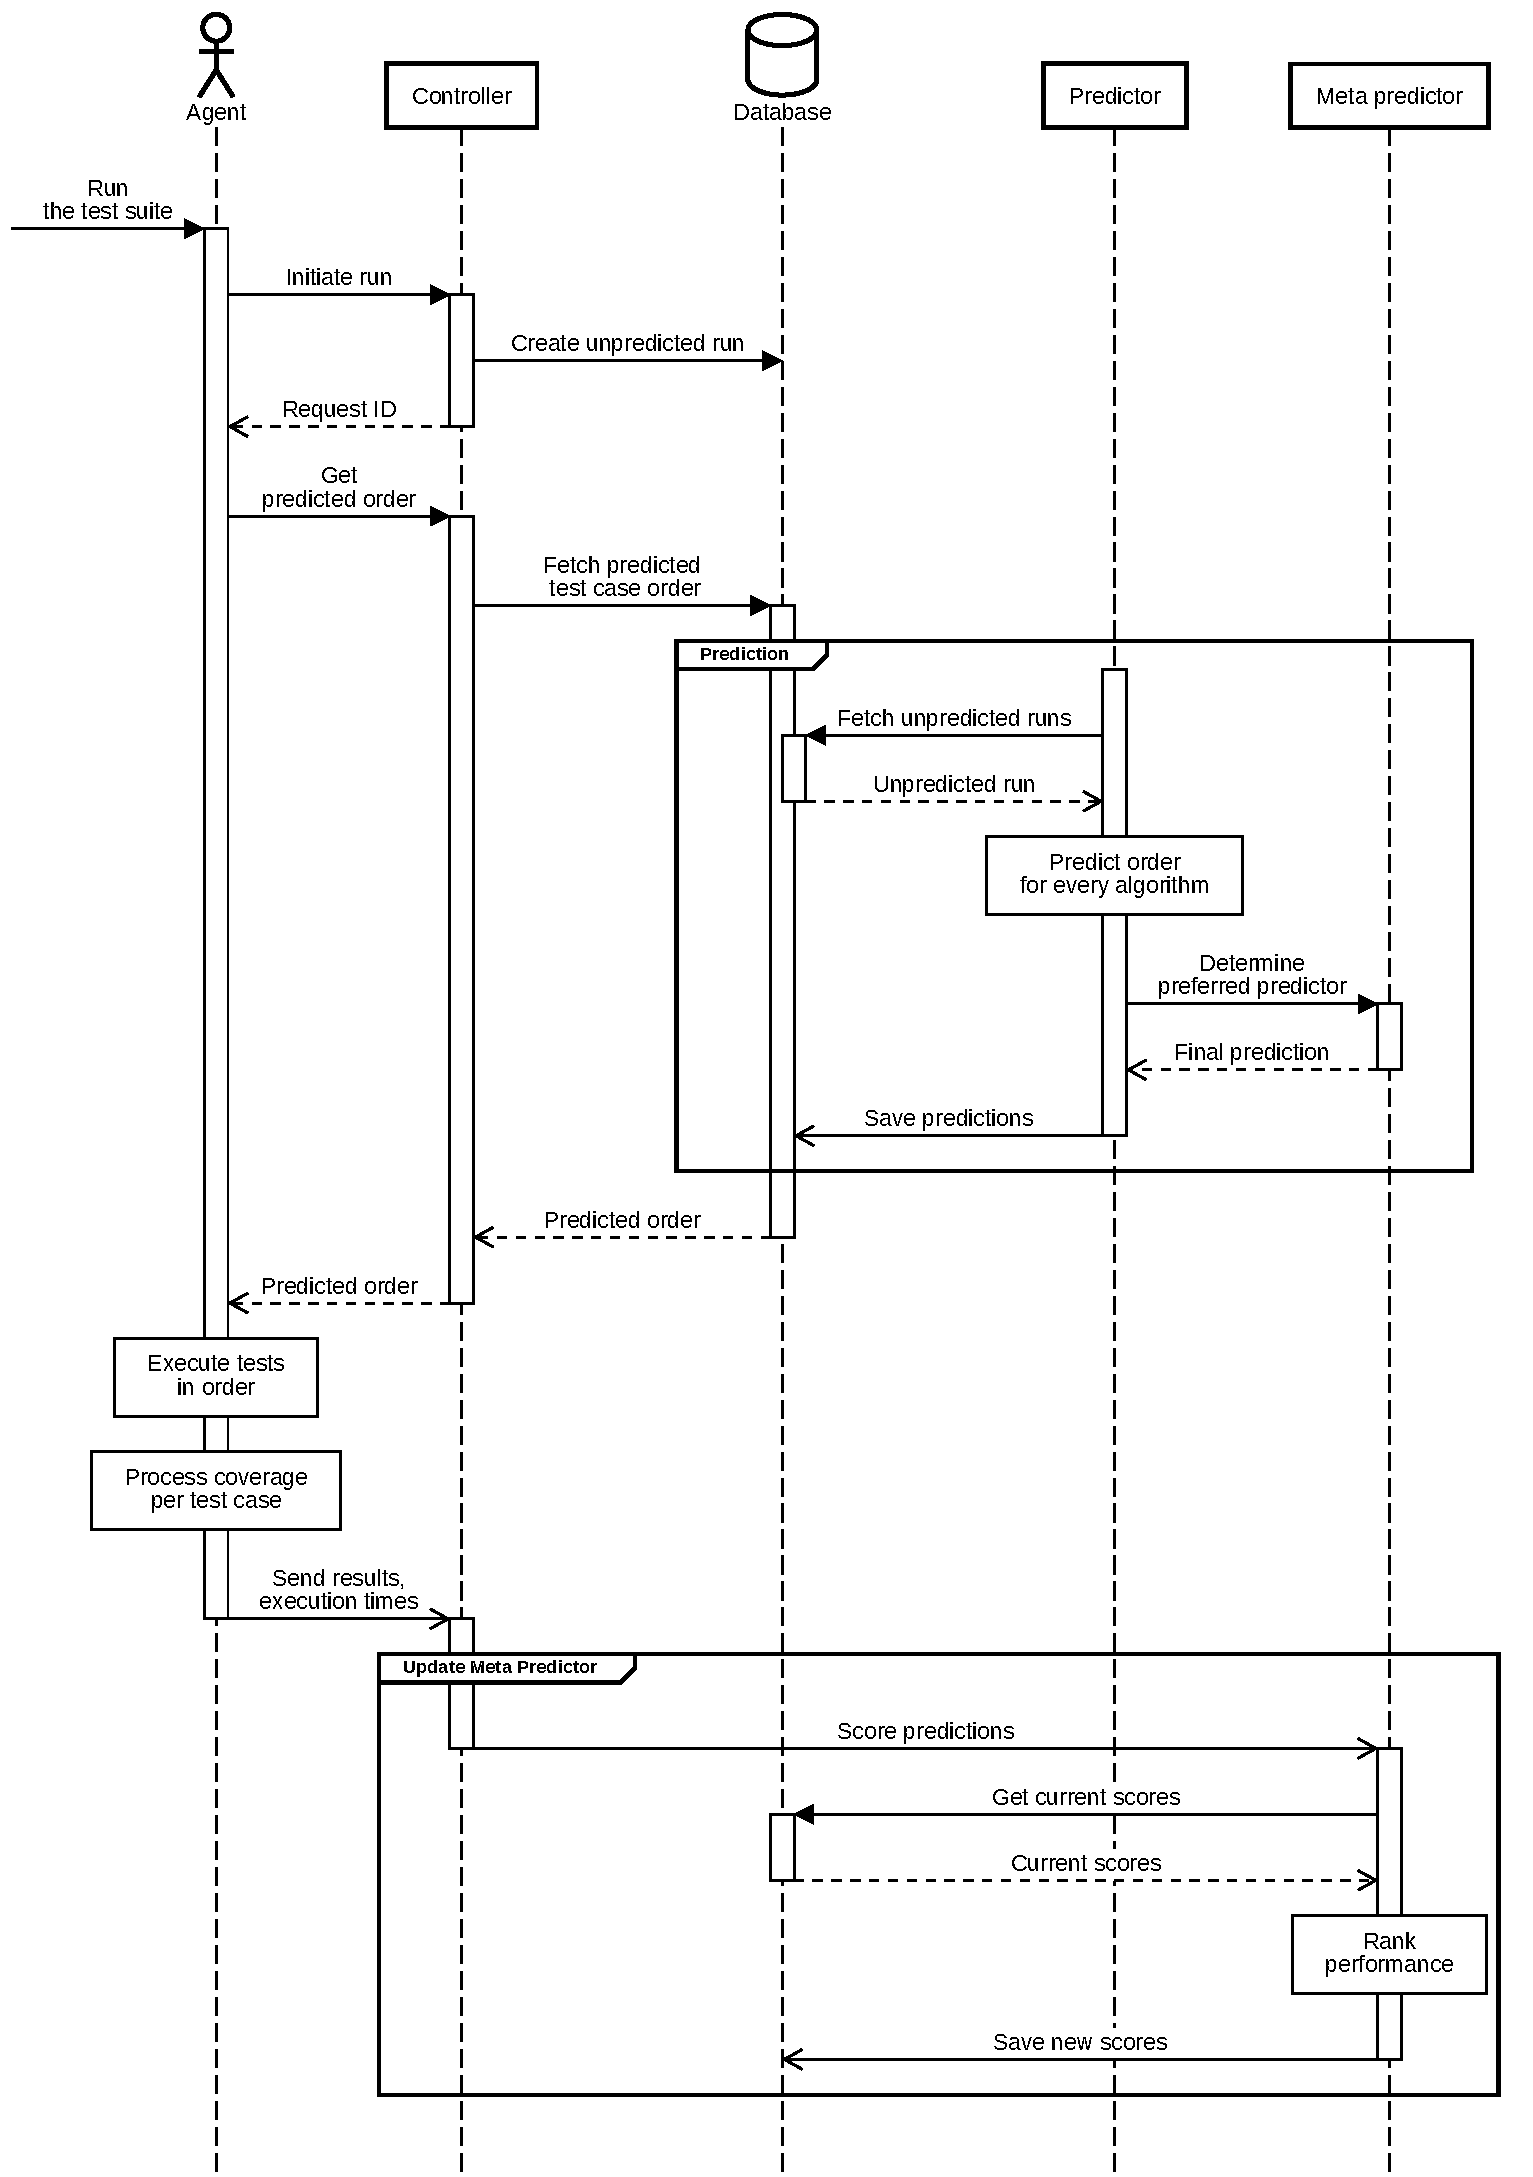
\includegraphics[height=\textheight]{assets/diagrams/sequence-diagram.pdf}
	\caption{Sequence diagram of \velocity{}}
	\label{fig:velocity-sequence-diagram}
\end{figure}

\subsection{Agent}
\label{ssec:velocity-frontend}
The first component that we will consider is the agent. The agent interacts directly with the source code and the test suite and is, therefore, the only component that is specific to the programming language and the test framework. Every programming language and test framework requires a different implementation of the agent, although these implementations are strongly related. This thesis provides a Java agent, which is available as a plugin for the Gradle and JUnit test framework, a combination which has previously been described in \cref{ssec:relatedwork-gradle-junit}. When the test suite is started, the plugin will contact the controller (\cref{ssec:velocity-controller}) to obtain the prioritised test case order and subsequently execute the test cases in that order. Afterwards, the plugin will send a feedback report to the controller, where it is analysed.

\subsection{Controller}\label{ssec:velocity-controller}
The second component is the core of the framework, acting as an intermediary between the agent on one side and the predictor (\cref{ssec:velocity-predictor}) on the other side. In order to satisfy the second design goal and as such allow language agnosticism, the controller exposes a \Gls{rest}-interface, to which the agent can communicate using the \texttt{HTTP} protocol. On the other side, the controller does not communicate directly with the predictor but stores prediction requests in a shared database instead. The predictor will periodically poll this database and update the request with the predicted order. Besides providing routing functionality between the agent and the predictor, the controller is additionally responsible for updating the meta predictor (\cref{ssec:pipeline-postanalysis}) by evaluating the accuracy of earlier predictions.

\subsection{Predictor and Metrics}\label{ssec:velocity-predictor}
The final component is the predictor. The predictor is responsible for applying the prioritisation algorithms to predict the optimal execution order of the test cases. This order is calculated by first executing ten prioritisation algorithms and subsequently consulting the meta predictor to determine the preferred sequence. The predictor has been implemented in Python, because of its accessibility and compatibility with various existing libraries such as NumPy\footnote{\url{https://numpy.org/}} and TensorFlow\footnote{\url{https://www.tensorflow.org/}}, to allow advanced prioritisation algorithms. 